\documentclass{article}

% Language setting
% Replace `english' with e.g. `spanish' to change the document language
\usepackage[english]{babel}

% Set page size and margins
% Replace `letterpaper' with `a4paper' for UK/EU standard size
\usepackage[letterpaper,top=2cm,bottom=2cm,left=3cm,right=3cm,marginparwidth=1.75cm]{geometry}

% Useful packages
\usepackage{amsmath}
\usepackage{graphicx}
\usepackage[colorlinks=true, allcolors=blue]{hyperref}

\title{PS6}
\author{Jack Wang}

\begin{document}
\maketitle



\section{Steps to clean the data}
\begin{enumerate}
\item Step1

Import data as tibble and merge data using sqldf;

\item Step2

Replace missing values in mgr\_exclude with 0, because firms that have missing value for this variable are highly likely those do not make Non-Gaap disclosure;

\item Step3

Rename two columns for simplicity

\item Step4

This is an ex post step, because I noticed there are outliers when I plot the eps and ARC. Winsorize eps and ARC column at 0.01 level.

\end{enumerate}


\section{Explanation of the images}

\subsection{PS6a}
This is a histogram of variable ng, which is a dummy variable indicating whether firms made Non-Gaap disclosure for that period. Histogram helps us to know the distribution of numbers of firms that made Non-Gaap disclosure in each year. It seems that the number of firms that made Non-Gaap disclosure each year is quite evenly distributed. The decrease in year 2019 is due to data availability. 
\begin{figure}[htp]
    \centering
    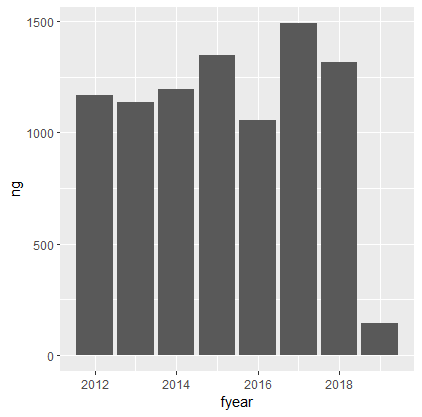
\includegraphics[width=4cm]{PS6a_Wang.png}
    \caption{Histogram of NG distribution}
    \label{fig:hist}
\end{figure}

\subsection{PS6b}
This is a point plot with fitted line to examine the trend of Non-Gaap eps across time. It seems that the disclosed eps is increasing over time.
\begin{figure}[htp]
    \centering
    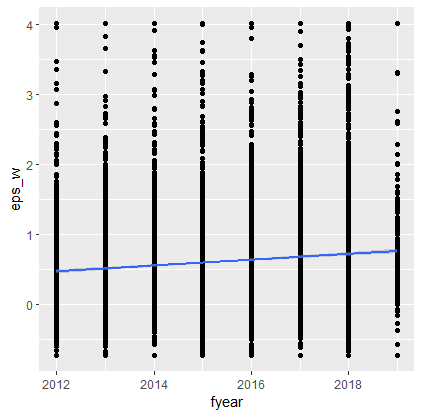
\includegraphics[width=4cm]{PS6b_Wang.png}
    \caption{EPS Trends}
    \label{fig:EPS trends}
\end{figure}

\subsection{PS6c}
This plot is to show how the Non-Gaap eps changes with ARC. I expect that with the increase in accounting reporting complexity (ARC), firms will report higher Non-Gaap eps. The plot generally documents this tendency, the fitted line has a positive slope.

\begin{figure}[htp]
    \centering
    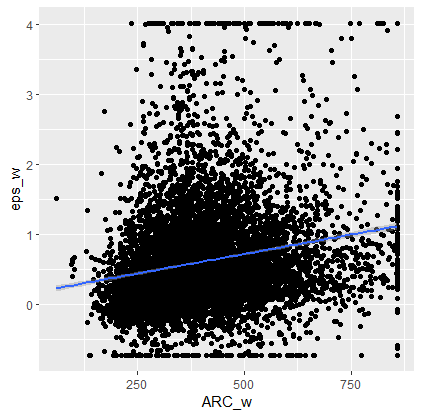
\includegraphics[width=4cm]{PS6c_Wang.png}
    \caption{How does ARC affect Non-Gaap EPS}
    \label{fig:ARC vs EPS}
\end{figure}

\subsection{PS6d}
This image shows how the ARC affect the Non-Gaap disclosure decision. The image indicates that higher ARC is associated with higher probability of Non-Gaap disclosure as expected.

\begin{figure}[htp]
    \centering
    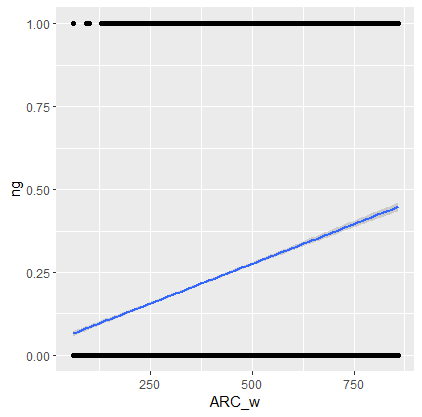
\includegraphics[width=4cm]{PS6d_Wang.png}
    \caption{How does ARC affect Non-Gaap disclosure decision}
    \label{fig:ARC vs NG}
\end{figure}

\end{document}